\documentclass{article}
\usepackage[utf8]{inputenc}
\usepackage{float}
\usepackage{hyperref}
\usepackage{pgfplots}
\pgfplotsset{width=10cm,compat=1.9}
\begin{document}

\title{Comparison of Containerized and Native Applications in the Store}
\author{Zac Freeman\\\\Reviewers:\\Paul Wiersma\\ Wesley Colin Wright}

\maketitle

\section{Introduction}
This document aims to summarize the costs and benefits of deploying Envoy to the stores using Docker containers as a part of Retail Acceleration. The purpose and resource overhead of containerizing Envoy within the Data Sync prototype will be discussed and analyzed in Resource Consumption, Latency, and Deployment Process. The utility and relevance of Docker to the store ecosystem will be discussed in Development Experience. Any code, data, or assumptions used in the analyses will be listed in Methodology, Data, and Scripts.

\section{Expected Outcomes}
The goals of this document are to
\begin{enumerate}
    \item Inform Architecture's decision on containerizing Envoy and other applications, within the scopes of the Retail Acceleration Data Sync prototype and final product
    \item Inform Architecture's future decisions on containerizing store applications by providing an approximation of the resource overhead of containerizing other store applications
\end{enumerate}

\section{Resource Consumption}
The foundation of the Docker container is the Linux namespace. A Linux namespace encapsulates a process to scope its access to system resources. A Docker container is able to make use of the host's kernel and additionally provide the dependencies needed by the containerized software in a virtual environment. This approach provides a lightweight solution to software virtualization.

The resource consumption of a containerized application is broken up into two groups. The first group, labelled "Docker Dependencies", consists of the per-system applications such as the docker daemon, the container daemon, etc., that support any number of containerized applications. The other group, labelled "Containerized Application", consists of the container and the application itself, which gives an approximation of the per-application cost of containerizing an application in the store.

\subsection{Storage Consumption}
The storage consumption was recorded while the applications were idle, under the assumption that putting the applications under load would not impact their installed size.

\begin{table}[H]
\begin{tabular}{ |c|c|c|c| }
 \hline
   & Storage (MB)\\ 
 \hline
 Native Application & 93.9 \\
 \hline
 Containerized Application & 84.6 \\
 \hline
 Docker Dependencies & 359.4\\
 \hline\hline
 Increase (with Dependencies) & 350.1 \\
 \hline
 Increase (without Dependencies) & -9.3 \\
 \hline
\end{tabular}
\caption{The storage consumed by the native Envoy application and the containerized Envoy application.}
\label{storage-consumption}
\end{table}

The decrease in storage costs between the native application and the containerized application is likely the result of the docker container using a version of the Envoy application compiled without debugging symbols, rather than some efficiency provided by Docker. The takeaway here is that containerizing Envoy represented a negligible increase in storage consumption.

\subsection{Memory Consumption}
The following plot was constructed from data collected while the Native and Containerized Applications were under simulated loads of 0, 10, 20, and 30 requests per second.

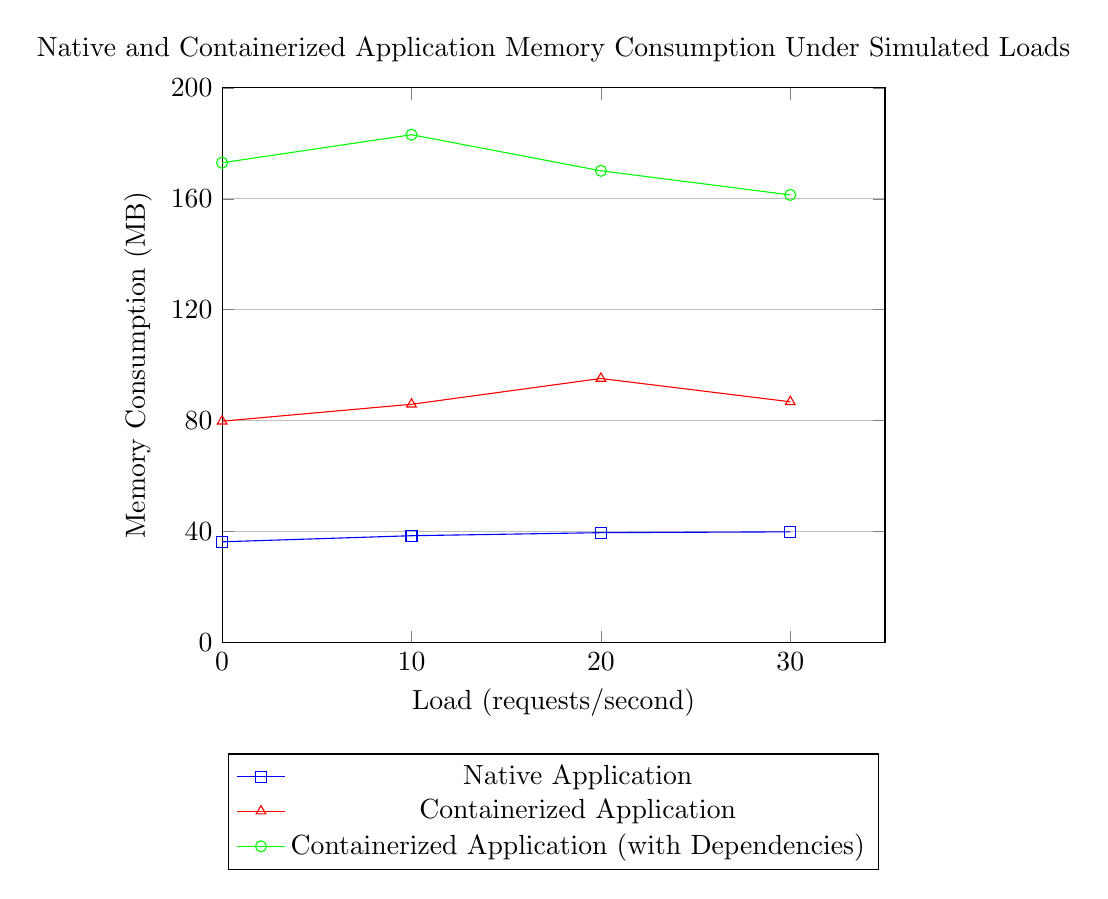
\begin{tikzpicture}
\begin{axis}[
    title={Native and Containerized Application Memory Consumption Under Simulated Loads},
    xlabel={Load (requests/second)},
    ylabel={Memory Consumption (MB)},
    xmin=0, xmax=35,
    ymin=0, ymax=200,
    xtick={0,10,20,30},
    ytick={0,40,80,120,160,200},
    legend style={at={(0.5,-0.2)},anchor=north},
    ymajorgrids=true,
]

\addplot[
    color=blue,
    mark=square,
    ]
    coordinates {
        (0, 36.3)(10, 38.5)(20, 39.6)(30, 39.9)
    };
    \addlegendentry{Native Application}

\addplot[
    color=red,
    mark=triangle,
    ]
    coordinates {
        (0, 79.8)(10, 85.9)(20, 95.2)(30, 86.8)
    };
    \addlegendentry{Containerized Application}
\addplot[
    color=green,
    mark=o,
    ]
    coordinates {
        (0, 173)(10, 183.1)(20, 170.1)(30, 161.4)
    };
    \addlegendentry{Containerized Application (with Dependencies)}
\end{axis}
\end{tikzpicture}

The Containerized Application (with and without Docker Dependencies) represents a fixed cost with respect to load on the containerized Envoy application.

The apparent decrease in Memory Consumption of the Containerized Application with respect to load is a result of variability in the memory consumption measurements.

\subsection{CPU Consumption}
The following plot was constructed from data collected while the Native and Containerized Applications were under simulated loads of 0, 10, 20, and 30 requests per second.

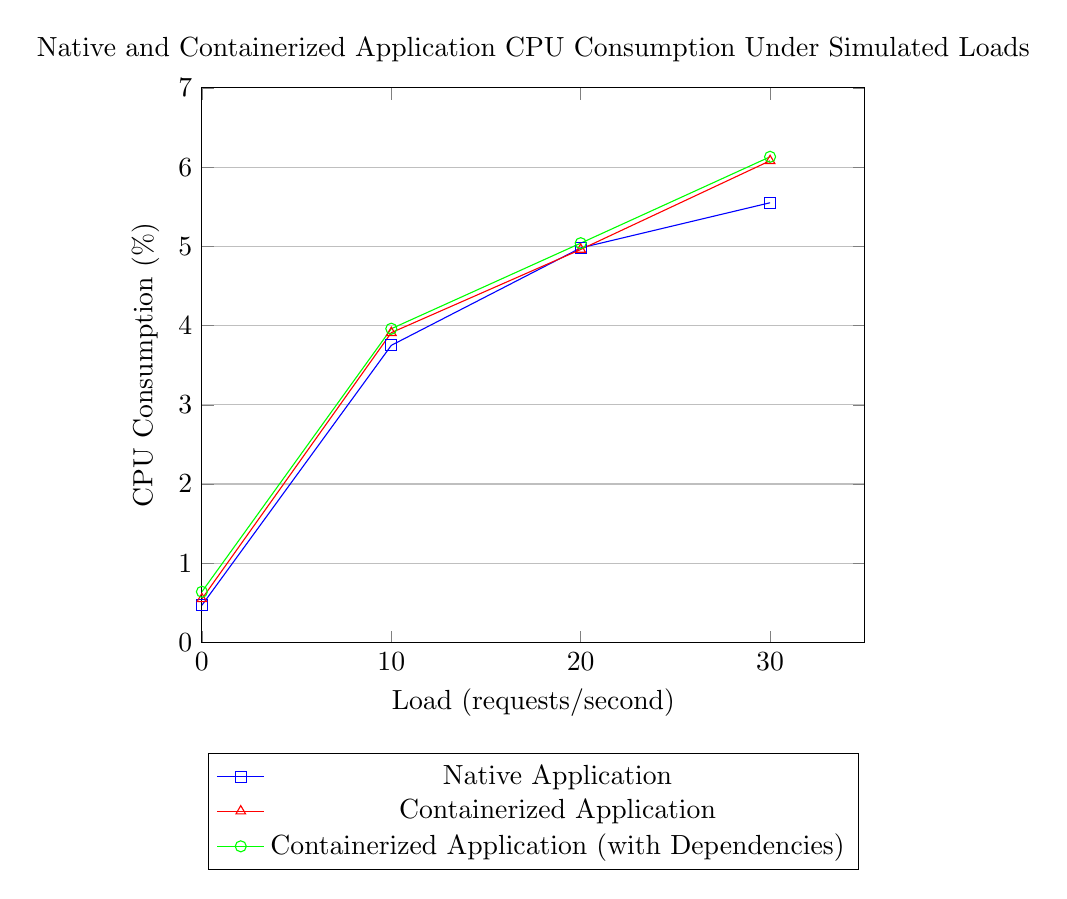
\begin{tikzpicture}
\begin{axis}[
    title={Native and Containerized Application CPU Consumption Under Simulated Loads},
    xlabel={Load (requests/second)},
    ylabel={CPU Consumption (\%)},
    xmin=0, xmax=35,
    ymin=0, ymax=7,
    xtick={0,10,20,30},
    ytick={0,1,2,3,4,5,6,7},
    legend style={at={(0.5,-0.2)},anchor=north},
    ymajorgrids=true,
]

\addplot[
    color=blue,
    mark=square,
    ]
    coordinates {
        (0, 0.47)(10, 3.75)(20, 4.98)(30, 5.55)
    };
    \addlegendentry{Native Application}

\addplot[
    color=red,
    mark=triangle,
    ]
    coordinates {
        (0, 0.55)(10, 3.91)(20, 4.96)(30, 6.08)
    };
    \addlegendentry{Containerized Application}
\addplot[
    color=green,
    mark=o,
    ]
    coordinates {
        (0, 0.64)(10, 3.96)(20, 5.04)(30, 6.13)
    };
    \addlegendentry{Containerized Application (with Dependencies)}
\end{axis}
\end{tikzpicture}

The Containerized Application (with and without Docker Dependencies) represent a small increase in CPU Consumption over the native Application.

The divergence at 30 requests/second is most likely a result of some variability in the method of measurement of CPU Consumption, but could warrant some more rigorous investigation.

\subsection{Interpretation}
Across the board, the containerized Envoy application requires more resources to run than the native Envoy application. Storage Consumption sees the greatest relative increase, followed by Memory Consumption, then CPU Consumption.

While the Storage Consumption of the Containerized Application (with Dependencies) represents a 4 fold increase over the native application, the increase in Storage Consumption is entirely due to the Docker Dependencies. The more containers that are running on the store, the smaller the relative increase in Storage Consumption becomes.

A similar observation can be made for the Memory Consumption of the Docker Dependencies - the more containers that are running on the store, the smaller the relative increase in Memory Consumption becomes. The remaining third of the increase in Memory Consumption, taken by the container, can potentially be optimized to a much smaller value.

The increase in CPU Consumption is regular, but small. The typical increase in CPU Consumption between the Native Application and the Containerized Application (with Docker Dependencies) is about 5 times smaller than the CPU Consumption of the Native Application when idle.

Furthermore, each of these increases in resource consumption do not scale with the load on the application. That is, containerizing an application represents a static resource cost with respect to load.

\section{Latency}
As mentioned in Resource Consumption, containers leverage the host's processes to minimize the cost of encapsulating an application. Reusing the host's network interface provides the additional benefit of reducing the latency introduced by the container.

\subsection{Results}
The following plot was constructed from data collected while the Native and Containerized Applications were under simulated loads of 0, 10, 20, and 30 requests per second, in addition to the requests made in order to survey their average response times.

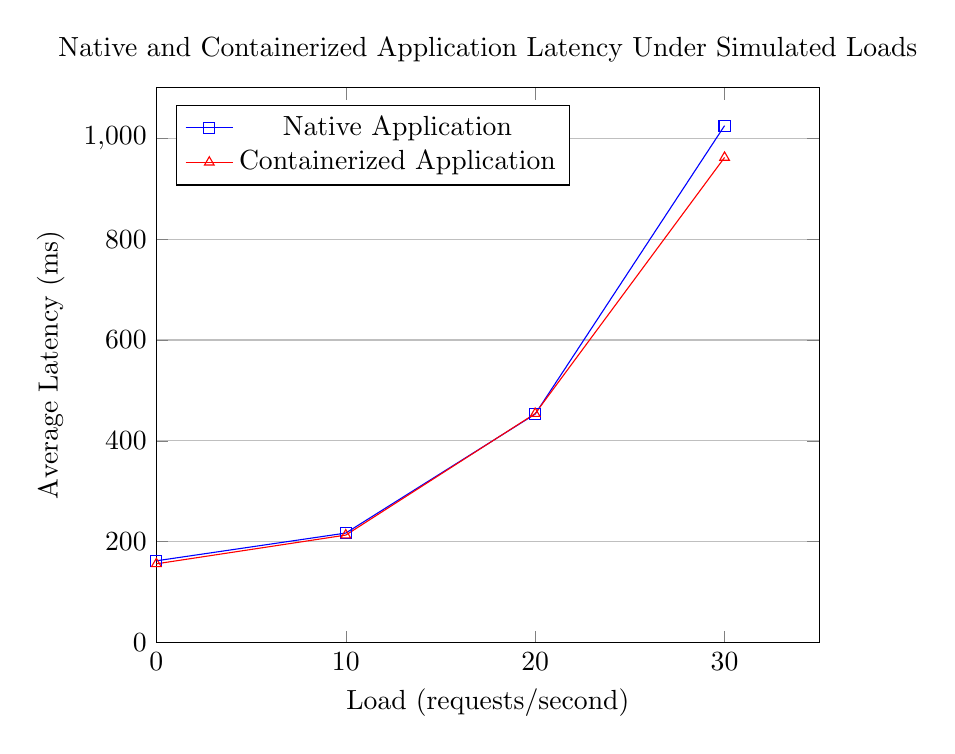
\begin{tikzpicture}
\begin{axis}[
    title={Native and Containerized Application Latency Under Simulated Loads},
    xlabel={Load (requests/second)},
    ylabel={Average Latency (ms)},
    xmin=0, xmax=35,
    ymin=0, ymax=1100,
    xtick={0,10,20,30},
    ytick={0,200,400,600,800,1000},
    legend pos=north west,
    ymajorgrids=true,
]

\addplot[
    color=blue,
    mark=square,
    ]
    coordinates {
        (0, 162)(10, 217)(20, 453)(30,1025)
    };
    \addlegendentry{Native Application}

\addplot[
    color=red,
    mark=triangle,
    ]
    coordinates {
        (0, 156)(10, 213)(20, 454)(30,962)
    };
    \addlegendentry{Containerized Application}
\end{axis}
\end{tikzpicture}

Under each simulated load, the difference between the average latencies of the Native and Containerized Applications was well within the standard deviation of each average latency. The negative increase in latency from the Containerized Application represents an insignificant difference in the calculated average latencies.

\subsection{Interpretation}
The containerized Envoy application does not incur a measurable increase in response times over the native Envoy application.

While the trend in the difference in latencies is promising, the trend of the latencies themselves are concerning. The underlying cause of the superlinear increase in average latency should be investigated to determine if components of the Data Sync prototype need to be reconsidered to meet the needs of the store.

\section{Deployment Process}
Currently, the Z-neXt project employs Docker to manage a containerized Envoy application. Envoy routes requests from in-store applications to either an above-store or in-store service, depending on the health of the above-store service.

\subsection{Container Deployment}
Deploying the Envoy container to a store requires that the Docker daemon be installed in the store and the official Envoy Docker image be downloaded from Docker Hub. Installing the Docker daemon necessitates enabling the \texttt{ol7\_addons-prod} package repository in the store. Once the image is downloaded to the store, it can be started by the Docker daemon.

This solution could be made production-ready by hosting the Docker image in the AutoZone Artifactory, and retrieving it in the store from the AutoZone Artifactory.

\subsection{Native Deployment}
Deploying the native Envoy application to a store would require adding the \texttt{tetrate-getenvoy} package repository to the store. Once the package repository is added, the Envoy application can be installed with the \texttt{getenvoy-envoy} package.

For the purposes of the Data Sync prototype, this proved too cumbersome a solution, as adding a new package repository (rather than just enabling an existing one) causes the \texttt{changeBranches} script to hang and fail. A resolution to this would involve the OS Conf team.

\section{Development Experience}
Docker provides a relatively approachable API for managing containers. Furthermore, Docker containers adhere to an industry-wide standard for containers, enabling easy transitions to other container management technologies.

\subsection{Loose Coupling}
By loosening the coupling between the store applications and the store system, containers enable developing, running, and testing a store application on a local machine, reducing the time between code change and application feedback and increasing developer productivity.

Furthermore, containerizing an application smooths its path towards running in the "cloud", if that option is pursued for the stores.

\subsection{Portability}
Containers simplify the process of running store applications outside of a store by packaging applications with their dependencies. Since an application's dependencies must be declared explicitly in the definition of its container, it becomes easier and more natural for a developer to state explicitly the dependencies of the applications they create. Encouraging the use of Docker for store applications would make each application more independent of a store's operating system and a store's configuration.

\subsection{Onboarding Acceleration}
Docker and containers provide a common language for environment configuration that can replace some of the domain-specific knowledge required to develop on the stores. This common language can accelerate the onboarding process of new store developers by standardizing parts of the process and leveraging developer's existing knowledge of Docker and containers.

\subsection{Reusability}
Containers, and their definitions, can be broken down into logical pieces called layers. This enables solutions to environment problems to be made once, stored in version control, and reused indefinitely by future applications.

\subsection{Reproducibility}
Containers enable much more of the store system's state can be encoded into version control, which makes more of said state reproducible and auditable.

\section{Methodology}
All scripts and commands were executed on \texttt{s8959.autozone.com}.

\subsection{Storage Consumption}
The size of each application was captured with \texttt{rpm -qi package\_name}. The size of the docker image used by the containerized application was captured from \texttt{docker images}.

\subsection{Memory Consumption}
The memory consumed by each process was equated with the physical memory being used by each process. The physical memory being used by each process was captured with \texttt{cat /proc/process\_id/status $|$ grep VmRSS}.

\subsection{CPU Consumption}
CPU consumption for each process was determined by taking the average of 100 values collected from \texttt{top} over a period of 200 seconds. \texttt{cpu-usage.sh} is used to collect these values and \texttt{stat-analysis.pl} is used to average the collected values.

While a standard deviation is produced for these collected values, it is not recorded as the average of the CPU usage is more akin to a single data point, than an average of data points. This is due to the extremely variable nature of the CPU usage of a process necessitating a series of measurements over time to approximate the expected CPU usage at one point in time.

\subsection{Latency}
Latency was measured by taking the average latency of 1000 requests to\\
\texttt{https://localhost:10443/v1/items/en-us} in 0.5 second intervals using\\
\texttt{latency-test.sh} to collect the latency values, and \texttt{stat-analysis.pl} to calculate the average and standard deviation of the collected values. Envoy was configured to route these requests to a local service to reduce the effects of variable network quality on the latency measurements.

\subsection{Load Testing}
To simulate various network loads on the envoy applications, \texttt{load-test.sh} was run to make 10, 20, or 30 requests per second to \texttt{https://localhost:10443/v1/items/en-us}. Envoy was configured to route these requests to a local service to avoid stressing the above store application.

\section{Data}
All data was collected from \texttt{s8959.autozone.com}.

\subsection{Storage Consumption}
The following data was collection while the Envoy application was idle.

The storage consumption listed for the Docker Dependencies represents the storage consumed by the packages added to use Docker in the store. This includes \texttt{docker-engine}, \texttt{docker-cli}, \texttt{containerd}, and \texttt{container-selinux}.

\begin{table}[H]
\begin{tabular}{ |c|c| }
 \hline
   & Storage (MB) \\ 
 \hline
 \texttt{docker-engine} & 103.7 \\
 \hline
 \texttt{docker-cli} & 168.7 \\
 \hline
 \texttt{containerd} & 87.0 \\
 \hline
 \texttt{container-selinux} & $<$0.1 \\
 \hline\hline
 Total & 359.4 \\
 \hline
\end{tabular}
\caption{A breakdown of the storage space consumed by each package that contributes to total storage consumption listed for the Docker Dependencies.}
\label{storage-breakdown}
\end{table}

The storage consumption listed for the Containerized Application is just the storage occupied by the Docker image used by the Envoy container. The storage consumption listed for the Native Application is just the storage occupied by the installed Envoy package.

\subsection{Memory and CPU Consumption}
The following data was collected while the Envoy application was under a simulated load of 0, 10, 20, and 30 requests per second.

The Memory and CPU consumption listed for the Docker Dependencies represents the memory and CPU time consumed by the applications required to support Docker containers in the store. This includes the \texttt{dockerd}, \texttt{containerd}, and \texttt{containerd-shim}.

The Memory and CPU consumption listed for the Containerized Application represents the memory and CPU time consumed by the Envoy application and the container that envelops it.

The Memory and CPU consumption listed for the Native Application represents just the memory and CPU time consumed by the native Envoy application.

\begin{table}[H]
\begin{tabular}{ |c|c|c| }
 \hline
   & Memory (MB) & CPU (\%) \\ 
 \hline
 Native Envoy & 36.3 & 0.47 \\
 \hline
 Containerized Envoy & 32.3 & 0.54 \\
 \hline
 Docker Container & 47.5 & 0.01 \\
 \hline
 \texttt{dockerd} & 75.1 & 0.05 \\
 \hline
 \texttt{containerd} & 10.8 & 0.03 \\
 \hline
 \texttt{containerd-shim} & 7.3 & 0.01 \\
 \hline\hline
 Native Application & 36.3 & 0.47 \\
 \hline
 Containerized Application & 79.8 & 0.55 \\
 \hline
 Docker Dependencies & 93.2 & 0.09 \\
 \hline\hline
 Increase (with Dependencies) & 136.7 & 0.17 \\
 \hline
 Increase (without Dependencies) & 43.5 & 0.08 \\
 \hline
\end{tabular}
\caption{A breakdown of the memory and CPU time consumed by the applications while idle.}
\label{idle-consumption-breakdown}
\end{table}

\begin{table}[H]
\begin{tabular}{ |c|c|c| }
 \hline
   & Memory (MB) & CPU (\%) \\ 
 \hline
 Native Envoy & 38.5 & 3.75 \\
 \hline
 Containerized Envoy & 38.9 & 3.90 \\
 \hline
 Docker Container & 47.0 & 0.01 \\
 \hline
 \texttt{dockerd} & 75.1 & 0.02 \\
 \hline
 \texttt{containerd} & 14.8 & 0.03 \\
 \hline
 \texttt{containerd-shim} & 7.3 & $<$0.01 \\
 \hline\hline
 Native Application & 36.3 & 3.75 \\
 \hline
 Containerized Application & 85.9 & 3.91 \\
 \hline
 Docker Dependencies & 97.2 & 0.05 \\
 \hline\hline
 Increase (with Dependencies) & 144.6 & 0.21 \\
 \hline
 Increase (without Dependencies) & 47.4 & 0.16 \\
 \hline
\end{tabular}
\caption{A breakdown of the memory and CPU time consumed by the applications while under a load of 10 requests per second.}
\label{consumption-breakdown-under-load-10}
\end{table}

\begin{table}[H]
\begin{tabular}{ |c|c|c| }
 \hline
   & Memory (MB) & CPU (\%) \\ 
 \hline
 Native Envoy & 39.6 & 4.98 \\
 \hline
 Containerized Envoy & 48.2 & 4.96 \\
 \hline
 Docker Container & 47.0 & $<$0.01 \\
 \hline
 \texttt{dockerd} & 54.3 & 0.06 \\
 \hline
 \texttt{containerd} & 13.1 & 0.02 \\
 \hline
 \texttt{containerd-shim} & 7.5 & $<$0.01 \\
 \hline\hline
 Native Application & 39.6 & 4.98 \\
 \hline
 Containerized Application & 95.2 & 4.96 \\
 \hline
 Docker Dependencies & 74.9 & 0.08 \\
 \hline\hline
 Increase (with Dependencies) & 130.5 & 0.06 \\
 \hline
 Increase (without Dependencies) & 55.6 & -0.02 \\
 \hline
\end{tabular}
\caption{A breakdown of the memory and CPU time consumed by the applications while under a load of 20 requests per second.}
\label{consumption-breakdown-under-load-20}
\end{table}

\begin{table}[H]
\begin{tabular}{ |c|c|c| }
 \hline
   & Memory (MB) & CPU (\%) \\ 
 \hline
 Native Envoy & 39.9 & 5.55 \\
 \hline
 Containerized Envoy & 39.9 & 6.08 \\
 \hline
 Docker Container & 46.9 & $<$0.01 \\
 \hline
 \texttt{dockerd} & 54.5 & 0.03 \\
 \hline
 \texttt{containerd} & 13.0 & 0.02 \\
 \hline
 \texttt{containerd-shim} & 7.1 & $<$0.01 \\
 \hline\hline
 Native Application & 39.9 & 5.55 \\
 \hline
 Containerized Application & 86.8 & 6.08 \\
 \hline
 Docker Dependencies & 74.6 & 0.05 \\
 \hline\hline
 Increase (with Dependencies) & 121.5 & 0.58 \\
 \hline
 Increase (without Dependencies) & 46.9 & 0.53 \\
 \hline
\end{tabular}
\caption{A breakdown of the memory and CPU time consumed by the applications while under a load of 30 requests per second.}
\label{consumption-breakdown-under-load-30}
\end{table}

The amount of memory consumed by the Envoy applications appear to grow with time when under load, and the memory consumed does not decrease when the simulated load is removed.

\subsection{Latency}
The following data was collected while the Envoy application was under a simulated load of 0, 10, 20, and 30 requests per second.

\begin{table}[H]
\begin{tabular}{ |c|c|c| }
 \hline
 & Average Latency (ms) & Standard Deviation (ms) \\
 \hline
 Native Application & 162 & 31 \\
 \hline
 Containerized Application & 156 & 39 \\
 \hline\hline
 Increase & -6 & \\
 \hline
\end{tabular}
\caption{A comparison of the applications' response times while idle.}
\label{idle-latency}
\end{table}

\begin{table}[H]
\begin{tabular}{ |c|c|c| }
 \hline
 & Average Latency (ms) & Standard Deviation (ms) \\
 \hline
 Native Application & 217 & 75 \\
 \hline
 Containerized Application & 213 & 72 \\
 \hline\hline
 Increase & -4 & \\
 \hline
\end{tabular}
\caption{A comparison of the applications' response times while under a load of 10 requests per second.}
\label{latency-under-load-10}
\end{table}

\begin{table}[H]
\begin{tabular}{ |c|c|c| }
 \hline
 & Average Latency (ms) & Standard Deviation (ms) \\
 \hline
 Native Application & 453 & 264 \\
 \hline
 Containerized Application & 454 & 278 \\
 \hline\hline
 Increase & 1 & \\
 \hline
\end{tabular}
\caption{A comparison of the applications' response times while under a load of 20 requests per second.}
\label{latency-under-load-20}
\end{table}

\begin{table}[H]
\begin{tabular}{ |c|c|c| }
 \hline
 & Average Latency (ms) & Standard Deviation (ms) \\
 \hline
 Native Application & 1025 & 640 \\
 \hline
 Containerized Application & 962 & 564 \\
 \hline\hline
 Increase & -63 & \\
 \hline
\end{tabular}
\caption{A comparison of the applications' response times while under a load of 30 requests per second.}
\label{latency-under-load-30}
\end{table}

It is interesting to note that standard deviations increase much more than the corresponding average latency when the applications are put under load, suggesting that the simulated load is causing a handful of requests to take much longer rather than causing all the requests to take slightly longer.

\section{Scripts}
The git repo containing these scripts (and the \latex for this document) can be found at \href{https://gitlab.autozone.com/10904928/docker-analysis}{https://gitlab.autozone.com/10904928/docker-analysis}.

\subsection{stat-analysis.pl}
\begin{verbatim}
#!/usr/bin/perl

use strict;

my @values = <>;

my $total = 0;
my $count = 0;
while (my $value = <@values>) {
    $total += $value;
    $count++;
}

my $average = $total / $count;
my $variance = 0;
while (my $value = <@values>) {
    $variance += ($value - $average)**2 / $count;
}

print "Average = ", $average, "\n";
print "Variance = ", $variance, "\n";
print "Standard Deviation = ", sqrt($variance), "\n";
\end{verbatim}

\subsection{cpu-usage.sh}
\begin{verbatim}
#!/bin/bash

if [[ $# -lt 2 ]]
then
    echo "missing arguments"
    exit
fi

pid="$1"
output="$2"
interval=1
num=100
if [[ $# -ge 3 ]]
then
    interval="$3"
fi

if [[ $# -eq 4 ]]
then
    num="$4"
fi

echo "recording CPU usage of process $pid $num times every 2*$interval seconds into $output..."

rm "$output"

for (( count=0; count<num; count++ ))
do
    top -b -n 2 -d "$interval" -p "$pid" | tail -1 | awk '{print $9}' >> "$output"
done
\end{verbatim}

\subsection{load-test.sh}
\begin{verbatim}
#!/bin/bash

if [[ $# -lt 1 ]]
then
    echo "missing url argument"
    exit
fi

url="$1"
interval=0.1
if [[ $# -eq 2 ]]
then
  interval="$2"
fi

echo "making requests to $url every $interval seconds..."

while true
do
    curl --insecure --silent --output "/dev/null" "$url" &
    sleep "$interval"
done
\end{verbatim}

\subsection{latency-test.sh}
\begin{verbatim}
#!/bin/bash

if [[ $# -lt 2 ]]
then
    echo "missing arguments"
    exit
fi

url="$1"
output="$2"
interval=0.5
num=100
if [[ $# -ge 3 ]]
then
    interval="$3"
fi

if [[ $# -eq 4 ]]
then
    num="$4"
fi

echo "recording response times for $num requests to $url made every $interval into $output..."

rm "$output"

for (( count=0; count<num; count++ ))
do
    curl --insecure --silent --output "/dev/null" --write-out "%{time_total}\n" "$url" >> "$output" &
    sleep "$interval"
done

\end{verbatim}

\end{document}
